\documentclass[13pt,a4paper]{extarticle}

% =========================================================================
% CẤU HÌNH TRANG VÀ LỀ THEO ĐÚNG QUY ĐỊNH CỦA GIẢNG VIÊN:
% Khổ giấy A4: Lề trên: 2.0 cm, Lề dưới: 2.0 cm, Lề trái: 3.0 cm, Lề phải: 2.0 cm
% =========================================================================
\usepackage[a4paper, top=2.0cm, bottom=2.0cm, left=3.0cm, right=2.0cm]{geometry}

% Phông chữ Times New Roman và hỗ trợ tiếng Việt chuẩn Unicode
\usepackage{fontspec}
\setmainfont{Times New Roman}

% Dãn dòng và dãn đoạn theo đúng quy định:
% Dãn dòng: 1.3; Thụt đầu dòng: 1 tab = 1.27 cm; Dãn đoạn trước/sau: 6pt
\usepackage{setspace}
\setstretch{1.3}
\setlength{\parindent}{1.27cm}
\setlength{\parskip}{6pt}

% Các gói toán học, đồ họa, bảng biểu và liên kết
\usepackage{amsmath, amssymb, amsfonts}
\usepackage{graphicx}
\usepackage{float}
\usepackage{booktabs}
\usepackage{tabularx}
\usepackage{multirow}
\usepackage{array}
\usepackage{caption}
\usepackage{xcolor}
\usepackage{tikz}
\usetikzlibrary{shapes.geometric, arrows.meta, positioning, calc, fit}
\usepackage[colorlinks=true, linkcolor=blue!80!black, citecolor=blue!80!black, urlcolor=blue!80!black]{hyperref}

% Đổi tên nhãn Bảng và Hình sang tiếng Việt chuẩn
\renewcommand{\tablename}{Bảng}
\renewcommand{\figurename}{Hình}

% Cấu hình tiêu đề Bảng và Hình theo đúng quy định:
% - Bảng: Tiêu đề đặt trên đầu bảng, in đậm, canh giữa
% - Hình: Tiêu đề đặt dưới hình, in đậm, canh giữa
\captionsetup[table]{
    position=top,
    justification=centering,
    font={bf},
    labelsep=period,
    skip=6pt
}
\captionsetup[figure]{
    position=bottom,
    justification=centering,
    font={bf},
    labelsep=period,
    skip=6pt
}

% Cấu hình định dạng đề mục (Heading) tối đa 3 cấp theo đúng quy định:
% 1. TIÊU ĐỀ CẤP 1 (IN HOA ĐẬM, CỠ CHỮ 13)
% 1.1. Tiêu đề cấp 2 (In đậm)
% 1.1.1. Tiêu đề cấp 3 (In đậm hoặc nghiêng)
\usepackage{titlesec}
\titleformat{\section}
  {\normalfont\fontsize{13}{16}\bfseries}{\thesection.}{0.5em}{\MakeUppercase}
\titlespacing*{\section}{0pt}{6pt}{6pt}

\titleformat{\subsection}
  {\normalfont\fontsize{13}{16}\bfseries}{\thesubsection.}{0.5em}{}
\titlespacing*{\subsection}{0pt}{6pt}{6pt}

\titleformat{\subsubsection}
  {\normalfont\fontsize{13}{16}\bfseries\itshape}{\thesubsubsection.}{0.5em}{}
\titlespacing*{\subsubsection}{0pt}{6pt}{6pt}

% =========================================================================
% BẮT ĐẦU NỘI DUNG TÀI LIỆU
% =========================================================================
\begin{document}

\pagenumbering{arabic}
\setcounter{page}{1}

% -------------------------------------------------------------------------
% TIÊU ĐỀ BÁO CÁO VÀ THÔNG TIN TÁC GIẢ THEO ĐÚNG MẪU QUY ĐỊNH CỦA GIẢNG VIÊN
% -------------------------------------------------------------------------
\begin{center}
    {\fontsize{13}{16}\selectfont \textbf{XÂY DỰNG HỆ THỐNG CHUYỂN VĂN BẢN TIẾNG VIỆT THÀNH GIỌNG NÓI MỨC TỪ BẰNG PHƯƠNG PHÁP TỔNG HỢP GHÉP NỐI}}\\[10pt]
    {\fontsize{13}{16}\selectfont \textbf{Vương Quang Vinh* và Hồ Phúc Thịnh}}\\[6pt]
\end{center}
\begin{flushright}
    {\fontsize{11}{14}\selectfont \textit{*Tác giả liên hệ (email: vqvinhhttt2211029@student.ctuet.edu.vn)}}
\end{flushright}
\vspace{6pt}

% -------------------------------------------------------------------------
% TÓM TẮT ĐỀ TÀI (ABSTRACT)
% -------------------------------------------------------------------------
\noindent\textbf{TÓM TẮT}\par
Báo cáo trình bày nghiên cứu và xây dựng hệ thống tổng hợp giọng nói từ văn bản tiếng Việt ở mức từ (Word-level Text-to-Speech) theo phương pháp tổng hợp ghép nối (Concatenative Speech Synthesis) trên nền tảng Cơ sở dữ liệu đa phương tiện. Mục đích của đề tài là tạo ra giọng đọc nghe rõ từng từ, đúng thanh điệu từ kho ngữ liệu âm thanh được thu âm thực tế. Câu đầu vào được chuẩn hóa, phân tách thành các từ đơn và mã hóa theo quy ước bộ gõ VNI; mã hóa này đóng vai trò là khóa định danh tra cứu nhanh trong cơ sở dữ liệu quan hệ SQLite nhằm lấy tệp âm thanh WAV tương ứng. Các tệp âm thanh được xử lý bằng các kỹ thuật xử lý tín hiệu số (DSP) chuyên sâu bao gồm cắt tỉa khoảng lặng động (Silence Trimming), chuẩn hóa năng lượng RMS, chèn khoảng nghỉ tự nhiên 120 ms và làm mờ chéo tuyến tính (Linear Cross-fade 10 ms) nhằm triệt tiêu tiếng nổ tại ranh giới ghép nối. Hệ thống được xây dựng hoàn chỉnh dưới dạng ứng dụng Web với backend FastAPI và frontend ReactJS SPA, cung cấp đầy đủ các chức năng: phòng tổng hợp thời gian thực, quản lý tra cứu 7.188 từ vựng và trực quan hóa 5 nhóm đặc trưng âm học số (Waveform, RMS, ZCR, cao độ $F_0$ và 13 hệ số MFCC). Kết quả thực nghiệm cho thấy hệ thống hoạt động ổn định, giọng đọc rõ ràng, bảo toàn nguyên vẹn sáu thanh điệu tiếng Việt và tốc độ phản hồi siêu tốc với hệ số thời gian thực $\text{RTF} < 0{,}04$.

\vspace{6pt}
\noindent\textbf{Từ khóa}: \textit{Chuyển văn bản thành giọng nói (TTS), Tổng hợp ghép nối, Cơ sở dữ liệu đa phương tiện, Xử lý tín hiệu số, VNI Encoding, SQLite, FastAPI, ReactJS.}

\vspace{12pt}

% -------------------------------------------------------------------------
% CÁC PHẦN CHÍNH CỦA BÁO CÁO (MODULAR INCLUSIONS)
% -------------------------------------------------------------------------
\section{ĐẶT VẤN ĐỀ}

Tổng hợp tiếng nói từ văn bản (Text-to-Speech, viết tắt là TTS) là một trong những bài toán nền tảng thuộc lĩnh vực xử lý ngôn ngữ tự nhiên (NLP) và xử lý tín hiệu đa phương tiện, nhằm chuyển đổi tự động một thông điệp văn bản dưới dạng ký tự số sang tín hiệu sóng âm thanh tương ứng có thể nghe và hiểu được (Dutoit, 1997). Trong kỷ nguyên số hóa và trí tuệ nhân tạo hiện nay, công nghệ TTS giữ vai trò cốt lõi trong việc xây dựng giao diện tương tác người -- máy bằng giọng nói (Voice User Interface - VUI), hỗ trợ đắc lực cho người khiếm thị tiếp cận tri thức số, tích hợp vào các hệ thống tổng đài phản hồi thông minh (IVR), đọc sách điện tử và tin tức báo chí tự động, cũng như tạo giọng nói tương tác cho các trợ lý ảo thông minh (Taylor, 2009).

Trong khuôn khổ học phần Cơ sở dữ liệu đa phương tiện, dữ liệu âm thanh (Audio) và văn bản (Text) đại diện cho hai đối tượng dữ liệu phi cấu trúc và bán cấu trúc tiêu biểu (Subrahmanian, 1998). Một hệ thống TTS toàn diện không chỉ đơn thuần giải quyết bài toán phát âm mà còn là bài toán thiết kế hệ thống quản trị cơ sở dữ liệu đa phương tiện: từ khâu tổ chức lưu trữ ngữ liệu song song (Parallel Audio-Text Corpus), trích xuất và lập chỉ mục các đặc trưng âm học số (Acoustic Feature Extraction and Indexing), cho đến việc tối ưu hóa truy vấn thời gian thực nhằm phục vụ tổng hợp tín hiệu mượt mà.

Đối với ngôn ngữ tiếng Việt, việc xây dựng hệ thống TTS phải đối mặt với nhiều thách thức mang tính chất âm học và ngôn ngữ học đặc thù:
\begin{enumerate}
    \item \textbf{Hệ thống thanh điệu phức tạp}: Tiếng Việt là một ngôn ngữ đơn lập có thanh điệu (Tonal language), bao gồm 6 thanh điệu cơ bản: Ngang (không dấu), Sắc, Huyền, Hỏi, Ngã và Nặng (Nguyễn Hữu Quỳnh, 2001). Thanh điệu trong tiếng Việt đóng vai trò khu biệt ngữ nghĩa sâu sắc: cùng một tổ hợp âm vị (ví dụ: \textit{ma, má, mà, mả, mã, mạ}) nhưng khi gắn với các thanh điệu khác nhau sẽ tạo thành các từ hoàn toàn khác biệt. Do đó, việc mã hóa chính xác thanh điệu là điều kiện tiên quyết để hệ thống tra cứu đúng bản ghi âm thanh tương ứng trong cơ sở dữ liệu.
    \item \textbf{Hiện tượng gián đoạn âm học tại ranh giới ghép nối}: Trong phương pháp tổng hợp ghép nối (Concatenative Speech Synthesis), các mẩu âm thanh độc lập được thu âm riêng rẽ khi ghép liên tiếp vào nhau sẽ xuất hiện sự gián đoạn đột ngột về pha tín hiệu (Phase discontinuity) và độ chênh lệch mức năng lượng (RMS energy mismatch) (Hunt và Black, 1996). Sự nhảy vọt biên độ tức thời này dẫn đến hiện tượng phát sinh tiếng nổ lách tách (click) hoặc tiếng bụp (pop), làm giảm sút nghiêm trọng chất lượng trải nghiệm của người nghe.
    \item \textbf{Ngữ điệu câu và hiện tượng đồng cấu âm (Coarticulation)}: Trong lời nói tự nhiên liên tục, các âm vị kế cận có xu hướng ảnh hưởng lẫn nhau do quán tính chuyển động liên tục của các bộ phận trong khoang miệng (môi, lưỡi, thanh môn) (Rabiner và Schafer, 2010). Việc ghép nối các đơn vị từ độc lập thường khiến ngữ điệu câu có cảm giác rời rạc, thiếu sự mượt mà và biến điệu tự nhiên của ngữ điệu tiếng Việt.
\end{enumerate}

Về phương pháp tổng hợp, lịch sử phát triển của công nghệ TTS đã ghi nhận ba hướng tiếp cận chủ đạo:
\begin{itemize}
    \item \textit{Tổng hợp tham số hoặc mô phỏng bộ máy phát âm (Formant/Articulatory Synthesis)}: Điển hình bởi hệ thống Klatt synthesizer hoặc phương pháp LPC (Linear Predictive Coding). Phương pháp này mô hình hóa đường truyền âm thanh của con người bằng các tham số toán học (Dutoit, 1997). Mặc dù tốc độ sinh nhanh và dung lượng lưu trữ cực nhỏ, giọng nói tổng hợp thường mang tính chất máy móc (robotic), khô cứng và thiếu đi tính tự nhiên.
    \item \textit{Tổng hợp ghép nối (Concatenative Speech Synthesis)}: Tiếp cận bằng cách lưu trữ một kho ngữ liệu các đơn vị âm thanh được thu âm thực tế (như từ, âm tiết, diphone hoặc triphone), sau đó lựa chọn và ghép nối tuần tự các đoạn âm thanh này để tạo thành câu hoàn chỉnh (Taylor, 2009). Điểm mạnh vượt trội của phương pháp này là bảo toàn 100\% chất giọng thực tế của người nói, không làm suy giảm chất lượng qua vocoder nhân tạo, đồng thời không đòi hỏi hạ tầng tính toán GPU phức tạp.
    \item \textit{Tổng hợp dựa trên mạng nơ-ron sâu (Neural/Deep Learning TTS)}: Tiêu biểu với các kiến trúc Tacotron 2, FastSpeech 2, hay VITS kết hợp neural vocoder (HiFi-GAN). Phương pháp này đem lại chất lượng ngữ điệu vượt bậc nhưng đòi hỏi kho ngữ liệu khổng lồ (hàng nghìn giờ âm thanh gán nhãn chi tiết) cùng năng lực tính toán phần cứng rất lớn để huấn luyện, không thích hợp cho các ứng dụng nhẹ triển khai tức thì trên thiết bị cục bộ.
\end{itemize}

Xuất phát từ yêu cầu học thuật của môn học Cơ sở dữ liệu đa phương tiện, nhóm nghiên cứu đã lựa chọn phương pháp \textbf{tổng hợp ghép nối mức từ (Word-level Concatenative TTS)} kết hợp với các kỹ thuật xử lý tín hiệu số (DSP) hiện đại. Đề tài tập trung vào việc tự xây dựng và quản trị kho ngữ liệu âm thanh thực nghiệm, thiết kế mô hình cơ sở dữ liệu quan hệ SQLite tối ưu hóa chỉ mục, đồng thời nghiên cứu giải thuật trích xuất các đặc trưng âm học số bao gồm: năng lượng RMS, tần suất cắt qua điểm không (ZCR), cao độ $F_0$ qua tự tương quan và 13 hệ số Cepstral trên thang tần số Mel (MFCCs).

Tính mới và giá trị ứng dụng của đề tài thể hiện ở việc:
\begin{enumerate}
    \item Xây dựng bộ quy ước mã hóa VNI hai chiều (Bidirectional VNI Encoding) độc lập với bảng mã Unicode, giải quyết triệt để sự phức tạp của ký tự tiếng Việt có dấu và cho phép tra cứu bản ghi đa phương tiện với tốc độ $O(1)$.
    \item Thiết kế và cài đặt thuật toán ghép nối mượt mà sử dụng kết hợp cắt tỉa khoảng lặng động (Silence Trimming), chuẩn hóa năng lượng RMS đồng nhất, kiểm soát biên độ đỉnh (Peak Limiter), mô hình hóa khoảng nghỉ ngắt câu (Pause Duration Modeling 120 ms) và kỹ thuật làm mờ chéo tuyến tính (Linear Cross-fade 10 ms).
    \item Tích hợp đầy đủ các API RESTful bất đồng bộ hiệu năng cao (FastAPI) cùng giao diện Web hiện đại (React 18 Single Page Application), hỗ trợ trực quan hóa dạng sóng, đường cong cao độ $F_0$ và phổ MFCC trực tiếp trên trình duyệt.
\end{enumerate}

Mục tiêu cốt lõi của đề tài là hoàn thiện hệ thống VietVoice TTS đáp ứng trọn vẹn 7 tiêu chí đánh giá khắt khe của học phần Cơ sở dữ liệu đa phương tiện: (1) Ngữ liệu song song văn bản -- âm thanh; (2) Kỹ thuật tổng hợp TTS mức từ; (3) Khả năng nhận văn bản và xuất âm thanh trực tiếp; (4) Sơ đồ khối và quy trình xử lý 5 bước rõ ràng; (5) Trích xuất và quản lý đặc trưng âm học số; (6) Mô hình CSDL đa phương tiện quan hệ chuẩn hóa; và (7) Thực nghiệm, đánh giá chất lượng toàn diện.


\section{PHƯƠNG PHÁP NGHIÊN CỨU}

Hệ thống VietVoice TTS được thiết kế theo phương pháp tổng hợp ghép nối mức từ (Word-level Concatenative Synthesis), kết hợp mô hình cơ sở dữ liệu quan hệ đa phương tiện và các kỹ thuật xử lý tín hiệu số (DSP) nhằm bảo đảm chất lượng âm thanh phát ra tự nhiên, rõ ràng và phản hồi theo thời gian thực.

\subsection{Ngữ liệu và Thiết kế Cơ sở dữ liệu Đa phương tiện}

\subsubsection{Ngữ liệu thu âm và quy ước mã hóa VNI}
Ngữ liệu của đề tài bao gồm 7.188 từ tiếng Việt được quản lý qua tệp \texttt{metadata\_encoded.csv}, cùng 5.429 tệp âm thanh đơn kênh (mono) ở định dạng WAV PCM 16-bit với tần số lấy mẫu chuẩn 22.050 Hz. Toàn bộ âm thanh được thu âm thực tế, giữ nguyên chất lượng âm học gốc của người đọc.

Để hệ thống tra cứu độc lập với bảng mã Unicode và không bị lỗi đường dẫn tệp trên các hệ điều hành, nhóm nghiên cứu xây dựng quy ước mã hóa hai chiều dựa trên bộ gõ VNI. Dấu thanh được chuyển thành chữ số từ 0 đến 5 đặt ở cuối mã từ (Bảng 1), còn các nguyên âm có dấu nón, dấu móc hoặc phụ âm gạch ngang được chuyển đổi thành ký tự ASCII đại diện (Bảng 2).

\begin{table}[H]
\centering
\caption{Quy ước mã hóa thanh điệu tiếng Việt}
\label{tab:tone_encoding}
\vspace{2pt}
\begin{tabular}{cclc}
\toprule
\textbf{Ký tự số} & \textbf{Tên thanh điệu} & \textbf{Ví dụ từ vựng} & \textbf{Mã hóa VNI} \\
\midrule
0 & Ngang (Không dấu) & ba, bay, anh & \texttt{ba0}, \texttt{bay0}, \texttt{anh0} \\
1 & Sắc & cá, bán, ánh & \texttt{ca1}, \texttt{ban1}, \texttt{anh1} \\
2 & Huyền & bà, bè, người & \texttt{ba2}, \texttt{be2}, \texttt{nguoi2} \\
3 & Hỏi & cảng, bả, hiểu & \texttt{cang3}, \texttt{ba3}, \texttt{hieu3} \\
4 & Ngã & bãi, vỗ, nghĩ & \texttt{bai4}, \texttt{vo+4}, \texttt{nghi4} \\
5 & Nặng & bạn, mẹ, thật & \texttt{ban5}, \texttt{me5}, \texttt{that5} \\
\bottomrule
\end{tabular}
\par\vspace{4pt}
\begin{minipage}{0.88\textwidth}
\fontsize{12}{14}\selectfont \textbf{Ghi chú}: Số đại diện thanh điệu luôn nằm ở cuối chuỗi mã để hệ thống dễ dàng bóc tách và đối sánh.\par
\textbf{Nguồn}: Đề xuất của nhóm nghiên cứu theo chuẩn VNI.
\end{minipage}
\end{table}

\begin{table}[H]
\centering
\caption{Quy ước mã hóa ký tự cấu trúc tiếng Việt}
\label{tab:char_encoding}
\vspace{2pt}
\begin{tabular}{lccccccc}
\toprule
\textbf{Ký tự gốc} & â & ă & ô & ơ & ê & ư & đ \\
\midrule
\textbf{Mã hóa VNI} & \texttt{a+} & \texttt{aa} & \texttt{o+} & \texttt{oo} & \texttt{e+} & \texttt{uu} & \texttt{d-} \\
\bottomrule
\end{tabular}
\par\vspace{4pt}
\begin{minipage}{0.88\textwidth}
\fontsize{12}{14}\selectfont \textbf{Ghi chú}: Các ký tự đặc biệt được ánh xạ sang tổ hợp ASCII nhằm tương thích tối đa với hệ thống tệp và CSDL.\par
\textbf{Nguồn}: Đề xuất của nhóm nghiên cứu.
\end{minipage}
\end{table}

Quy trình bóc tách và chuyển đổi từ vựng tiếng Việt sang mã định danh VNI được mô hình hóa trực quan qua lưu đồ trong Hình 1.

\begin{figure}[H]
\centering
\begin{tikzpicture}[
    startstop/.style={rectangle, rounded corners=6pt, text width=5.0cm, minimum height=0.8cm, text centered, draw=blue!70!black, fill=blue!10, font=\small\bfseries},
    process/.style={rectangle, rounded corners=3pt, text width=6.6cm, minimum height=0.8cm, text centered, draw=black!70, fill=gray!10, font=\small},
    branch/.style={rectangle, rounded corners=3pt, text width=3.4cm, minimum height=1.1cm, text centered, align=center, draw=teal!70!black, fill=teal!10, font=\small},
    arrow/.style={thick, -{Stealth[length=2.5mm]}, draw=black!75}
]
\node (in) [startstop] {Từ tiếng Việt (chuẩn NFC)};
\node (nfd) [process, below=0.8cm of in] {Phân rã chuỗi NFD (Tách dấu phụ)};
\node (split) [process, below=0.8cm of nfd] {Duyệt từng ký tự \& Phân loại};

% 3 nhánh rẽ ngang nhau, phân bố đối xứng rõ ràng
\node (struct) [branch, below=1.2cm of split] {\textbf{Ký tự cấu trúc}\\(â$\to$\texttt{a+}, ă$\to$\texttt{aa}, đ$\to$\texttt{d-})};
\node (base) [branch, left=0.8cm of struct] {\textbf{Ký tự cơ sở}\\(a, b, c,...)};
\node (tone) [branch, right=0.8cm of struct] {\textbf{Dấu thanh}\\(sắc$\to$1, huyền$\to$2,...)};

\node (merge) [process, below=1.2cm of struct, text width=8.2cm] {Ghép chuỗi: [Ký tự cấu trúc] + [Mã thanh điệu]};
\node (out) [startstop, below=0.8cm of merge, fill=teal!15, draw=teal!70!black, text width=6.8cm] {Mã VNI đại diện (ví dụ: \texttt{ca1}, \texttt{ban5})};

\draw [arrow] (in) -- (nfd);
\draw [arrow] (nfd) -- (split);
\draw [arrow] (split) -| (base.north);
\draw [arrow] (split) -- (struct.north);
\draw [arrow] (split) -| (tone.north);
\draw [arrow] (base.south) |- (merge);
\draw [arrow] (struct.south) -- (merge);
\draw [arrow] (tone.south) |- (merge);
\draw [arrow] (merge) -- (out);
\end{tikzpicture}
\caption{Lưu đồ thuật toán mã hóa từ tiếng Việt sang mã VNI}
\label{fig:vni_flowchart}
\par\vspace{4pt}
\begin{minipage}{0.88\textwidth}
\centering\fontsize{12}{14}\selectfont \textbf{Nguồn}: Mô hình hóa giải thuật từ hàm \texttt{encode\_word()} trong backend.
\end{minipage}
\end{figure}

\subsubsection{Thiết kế Cơ sở dữ liệu Đa phương tiện SQLite}
Kho ngữ liệu và các đặc trưng số được lưu trữ trong hệ quản trị cơ sở dữ liệu SQLite 3 với cấu trúc 4 bảng quan hệ chuẩn hóa (Bảng 3).

\begin{table}[H]
\centering
\caption{Cấu trúc các bảng trong cơ sở dữ liệu đa phương tiện VietVoice}
\label{tab:db_schema}
\vspace{2pt}
\begin{tabularx}{\textwidth}{p{3.0cm}p{3.8cm}X}
\toprule
\textbf{Tên bảng} & \textbf{Khóa chính / ngoại} & \textbf{Ý nghĩa và chức năng} \\
\midrule
\texttt{speakers} & \texttt{speaker\_id} (PK) & Quản lý danh mục người đọc, tên và mô tả giọng thu. \\
\addlinespace
\texttt{words} & \texttt{word\_id} (PK) & Danh mục từ vựng, từ gốc có dấu, mã \texttt{encoded\_word} và tên tệp mã hóa \texttt{encoded\_filename}. \\
\addlinespace
\texttt{audio\_records} & \texttt{audio\_id} (PK)\newline \texttt{word\_id} (FK)\newline \texttt{speaker\_id} (FK) & Lưu trữ đường dẫn tệp âm thanh WAV, kênh, tần số lấy mẫu (22.050 Hz), số khung, thời lượng và kích thước tệp. \\
\addlinespace
\texttt{audio\_features} & \texttt{feature\_id} (PK)\newline \texttt{audio\_id} (FK, UNIQUE) & Lưu trữ các đặc trưng số đã trích xuất: năng lượng RMS, biên độ đỉnh, ZCR, cao độ $F_0$, tỷ lệ hữu thanh, chuỗi JSON của 13 hệ số MFCC và dạng sóng rút gọn. \\
\bottomrule
\end{tabularx}
\par\vspace{4pt}
\begin{minipage}{\textwidth}
\fontsize{12}{14}\selectfont \textbf{Ghi chú}: Ràng buộc khóa ngoại \texttt{ON DELETE CASCADE} bảo đảm tính toàn vẹn giữa dữ liệu âm thanh và các vector đặc trưng.\par
\textbf{Nguồn}: Thiết kế hệ thống VietVoice TTS.
\end{minipage}
\end{table}

Hệ thống thiết lập các chỉ mục B-Tree trên trường \texttt{word} (bảng \texttt{words}) cùng các trường \texttt{word\_id} và \texttt{speaker\_id} (bảng \texttt{audio\_records}), giúp câu truy vấn ghép nối theo lô (\textit{batch query}) đạt tốc độ xấp xỉ $O(1)$, bảo đảm thời gian phản hồi dưới 100 ms ngay cả khi tổng hợp câu dài.

\subsection{Quy trình Xử lý Tín hiệu Số và Ghép nối Âm thanh (DSP Pipeline)}

Toàn bộ quy trình chuyển đổi từ một câu văn bản tiếng Việt sang dòng âm thanh WAV hoàn chỉnh được mô hình hóa chi tiết tại sơ đồ khối Hình 2.

\begin{figure}[H]
\centering
\begin{tikzpicture}[
    startstop/.style={rectangle, rounded corners=6pt, text width=6.8cm, minimum height=0.8cm, text centered, draw=blue!70!black, fill=blue!10, font=\small\bfseries},
    process/.style={rectangle, rounded corners=3pt, text width=8.5cm, minimum height=0.8cm, text centered, draw=black!70, fill=gray!10, font=\small},
    decision/.style={diamond, text width=3.2cm, minimum height=1.1cm, text centered, align=center, draw=orange!80!black, fill=orange!15, font=\small},
    warn/.style={rectangle, rounded corners=3pt, text width=3.2cm, minimum height=0.8cm, text centered, align=center, draw=red!70!black, fill=red!10, font=\small},
    arrow/.style={thick, -{Stealth[length=2.5mm]}, draw=black!75}
]
\node (start) [startstop] {1. Câu văn bản tiếng Việt đầu vào};
\node (p1) [process, below=0.7cm of start] {2. Chuẩn hóa Unicode NFC \& Phân tách token từ vựng};
\node (p2) [process, below=0.7cm of p1] {3. Mã hóa VNI \& Truy vấn CSDL SQLite theo lô};
\node (dec) [decision, below=0.9cm of p2] {Đủ tệp âm\\thanh WAV?};
\node (warn) [warn, right=1.6cm of dec] {Cảnh báo từ thiếu\\(\textit{missing words})};
\node (p3) [process, below=0.9cm of dec] {4. Tiền xử lý DSP: Cắt khoảng lặng \& Chuẩn hóa RMS (9000)};
\node (p4) [process, below=0.7cm of p3] {5. Ghép nối: Chèn Pause 120 ms \& Cross-fade 10 ms};
\node (stop) [startstop, below=0.7cm of p4, fill=teal!15, draw=teal!70!black] {Xuất tệp WAV PCM 16-bit \& Dữ liệu Timeline};

\draw [arrow] (start) -- (p1);
\draw [arrow] (p1) -- (p2);
\draw [arrow] (p2) -- (dec);
\draw [arrow] (dec) -- node[above, font=\footnotesize\bfseries, text=red!80!black] {Không} (warn);
\draw [arrow] (dec) -- node[right, font=\footnotesize\bfseries, text=teal!80!black] {Có} (p3);
\draw [arrow] (p3) -- (p4);
\draw [arrow] (p4) -- (stop);
\end{tikzpicture}
\caption{Sơ đồ quy trình tổng hợp tiếng nói tuần tự và xử lý tín hiệu số}
\label{fig:tts_pipeline_diagram}
\par\vspace{4pt}
\begin{minipage}{0.88\textwidth}
\centering\fontsize{12}{14}\selectfont \textbf{Nguồn}: Mô hình hóa quy trình tổng hợp 5 bước của hệ thống VietVoice TTS.
\end{minipage}
\end{figure}

Trong quy trình trên, hai kỹ thuật xử lý tín hiệu số (DSP) giữ vai trò quyết định đến chất lượng âm thanh:
\begin{enumerate}
    \item \textbf{Cắt tỉa khoảng lặng (Silence Trimming) và Chuẩn hóa năng lượng RMS}: Tự động dò tìm các mẫu âm thanh có biên độ vượt ngưỡng nền 500 (trên thang PCM 16-bit) để cắt bỏ khoảng lặng thừa trước và sau phát âm; đồng thời điều chỉnh năng lượng hiệu dụng về mức chuẩn 9.000 kết hợp bộ giới hạn đỉnh (Peak Limiter tối đa 30.000) nhằm cân bằng độ to và tránh méo tiếng.
    \item \textbf{Chèn khoảng nghỉ (Pause Modeling) và Làm mượt biên giới từ (Linear Cross-fade)}: Chèn quãng nghỉ 120 ms giữa hai từ liên tiếp mô phỏng nhịp điệu nói tự nhiên. Tại điểm nối giữa hai mẩu âm thanh, hệ thống áp dụng kỹ thuật làm mờ chéo trong khoảng 10 ms (Hình 3): biên độ đoạn trước giảm dần (Fade-out) đồng thời biên độ đoạn sau tăng dần (Fade-in). Nhờ đó, tín hiệu số chuyển tiếp êm ái, xóa bỏ hoàn toàn tiếng nổ lách tách (click/pop) do gián đoạn pha gây ra.
\end{enumerate}

\begin{figure}[H]
\centering
\begin{tikzpicture}[x=1cm, y=1cm, every node/.style={font=\small}]

% ============================================================
% Layout hoàn toàn nằm ngang (horizontal), hai khối song song
% Từ thứ nhất: [0,5.5]  |  Overlap: [5.5,7.5]  |  Từ thứ hai: [5.5,13]
% Tất cả trung tâm cùng mức y=0, cao 1.4cm (y=-0.7 .. +0.7)
% ============================================================

% === Từ thứ nhất (trái, màu xanh dương) ===
\draw[thick, fill=blue!10, draw=blue!70!black, rounded corners=3pt]
    (0.0, -0.7) rectangle (7.5, 0.7);
\node[align=center] at (3.0, 0.0)
    {\textbf{Đoạn âm thanh}\\[2pt]\textbf{Từ thứ nhất} ($x_1$)};

% === Từ thứ hai (phải, màu xanh lá) ===
\draw[thick, fill=teal!10, draw=teal!70!black, rounded corners=3pt]
    (5.5, -0.7) rectangle (13.0, 0.7);
\node[align=center] at (10.0, 0.0)
    {\textbf{Đoạn âm thanh}\\[2pt]\textbf{Từ thứ hai} ($x_2$)};

% === Vùng chồng lặp Cross-fade [5.5, 7.5] ===
\fill[orange!18] (5.5, -1.1) rectangle (7.5, 1.4);
\draw[dashed, very thick, draw=orange!80!black] (5.5, -1.1) rectangle (7.5, 1.4);
\node[above=3pt, text=orange!90!black, font=\small\bfseries, align=center]
    at (6.5, 1.4) {Vùng Cross-fade\\(10 ms)};

% === Mũi tên Fade-out (chéo từ trên trái → xuống phải) ===
\draw[very thick, -{Stealth[length=3mm]}, red!80!black]
    (5.5, 0.55) -- (7.5, -0.3);
% Nhãn Fade-out đặt bên ngoài vùng overlap (bên trái, trên)
\node[left=3pt, font=\footnotesize\bfseries, text=red!80!black, align=right]
    at (5.5, 0.9) {Fade-out\\($1 - \alpha$)};

% === Mũi tên Fade-in (chéo từ dưới trái → lên phải) ===
\draw[very thick, -{Stealth[length=3mm]}, teal!70!black]
    (5.5, -0.55) -- (7.5, 0.3);
% Nhãn Fade-in đặt bên ngoài vùng overlap (bên trái, dưới)
\node[left=3pt, font=\footnotesize\bfseries, text=teal!70!black, align=right]
    at (5.5, -0.9) {Fade-in\\($\alpha$)};

% === Mũi tên xuống ===
\draw[very thick, -{Stealth[length=3.5mm]}, black!80]
    (6.5, -1.4) -- (6.5, -2.3);
\node[right=6pt, font=\small] at (6.5, -1.85)
    {$y[n] = (1-\alpha)\,x_1[n] + \alpha\,x_2[n]$};

% === Khung kết quả ===
\draw[thick, fill=teal!15, draw=teal!70!black, rounded corners=3pt]
    (0.5, -3.4) rectangle (12.5, -2.5);
\node[align=center, font=\small] at (6.5, -2.95)
    {\textbf{Tín hiệu âm thanh tổng hợp liền mạch}
     \enspace (Triệt tiêu tiếng nổ lách tách — click/pop)};

\end{tikzpicture}
\caption{Sơ đồ nguyên lý làm mượt biên giới từ bằng kỹ thuật Linear Cross-fade}
\label{fig:crossfade_diagram}
\par\vspace{4pt}
\begin{minipage}{0.92\textwidth}
\centering\fontsize{12}{14}\selectfont
\textbf{Nguồn}: Mô phỏng kỹ thuật làm mờ chéo từ hàm \texttt{concatenate()} trong backend (dòng 252--262).
\end{minipage}
\end{figure}

\subsection{Trích xuất Đặc trưng Âm thanh Số (Acoustic Feature Extraction)}

Bên cạnh chức năng tổng hợp, hệ thống xây dựng mô-đun phân tích đặc trưng âm học số \texttt{extract\_features.py} để phục vụ nghiên cứu và trực quan hóa trong môn học CSDL Đa phương tiện. Tín hiệu âm thanh được phân khung ngắn hạn (độ dài khung 1.024 mẫu, bước nhảy 256 mẫu, nhân cửa sổ Hanning) để trích xuất 5 nhóm thuộc tính cốt lõi theo lưu đồ Hình 4:
\begin{itemize}
    \item \textbf{Năng lượng hiệu dụng (RMS Energy) và Biên độ đỉnh (Peak Amplitude)}: Phản ánh độ to cảm nhận và mức cường độ tín hiệu lớn nhất của từ vựng.
    \item \textbf{Tần suất cắt qua điểm không (Zero-Crossing Rate - ZCR)}: Đếm số lần tín hiệu đổi dấu qua mức 0, là chỉ số kinh điển giúp phân biệt âm hữu thanh (ZCR thấp) và âm vô thanh (ZCR cao).
    \item \textbf{Cao độ cơ bản $F_0$ (Pitch)}: Ước lượng tần số rung động của dây thanh âm bằng thuật toán tự tương quan (\textit{Autocorrelation}) trên miền thời gian trong dải tần sinh học 50--500 Hz, đồng thời tính tỷ lệ khung hữu thanh (\textit{voiced fraction}).
    \item \textbf{13 Hệ số MFCC (Mel-Frequency Cepstral Coefficients)}: Trích xuất qua biến đổi phổ FFT, ngân hàng 26 bộ lọc tam giác Mel và biến đổi cosin rời rạc (DCT-II). 13 hệ số MFCC đại diện cho đường bao phổ và đặc trưng âm sắc vòm họng của người nói.
\end{itemize}

\begin{figure}[H]
\centering
\begin{tikzpicture}[
    startstop/.style={rectangle, rounded corners=6pt, text width=6.5cm, minimum height=0.8cm, text centered, draw=blue!70!black, fill=blue!10, font=\small\bfseries},
    process/.style={rectangle, rounded corners=3pt, text width=8.5cm, minimum height=0.8cm, text centered, draw=black!70, fill=gray!10, font=\small},
    feat/.style={rectangle, rounded corners=4pt, text width=3.3cm, minimum height=1.2cm, text centered, align=center, draw=purple!70!black, fill=purple!8, font=\small},
    arrow/.style={thick, -{Stealth[length=2.5mm]}, draw=black!75}
]
\node (in) [startstop] {Tệp âm thanh WAV PCM 16-bit (22.050 Hz)};
\node (prep) [process, below=0.7cm of in] {Phân khung ($N=1024, H=256$) \& Áp dụng cửa sổ Hanning};

% 4 khối đặc trưng phân bố ngang cân đối, không va chạm
\coordinate (center_level) at ([yshift=-1.2cm]prep.south);
\node (f2) [feat] at ([xshift=-1.9cm]center_level) {\textbf{Tần suất ZCR}\\(Âm hữu/vô thanh)};
\node (f1) [feat] at ([xshift=-5.6cm]center_level) {\textbf{Năng lượng RMS}\\\& Biên độ đỉnh Peak};
\node (f3) [feat] at ([xshift=1.9cm]center_level) {\textbf{Cao độ $F_0$}\\(Tự tương quan 50--500 Hz)};
\node (f4) [feat] at ([xshift=5.6cm]center_level) {\textbf{13 Hệ số MFCC}\\(Mel-filterbank + DCT)};

\node (save) [startstop, below=1.3cm of center_level, fill=teal!15, draw=teal!70!black, text width=12.5cm] {Đóng gói vector JSON \& Lưu trữ vào bảng \texttt{audio\_features} trong SQLite};

% Đường phân nhánh từ prep xuống 4 khối
\draw [arrow] (in) -- (prep);
\draw [thick, draw=black!75] (prep.south) -- ++(0,-0.4) coordinate (bus_top);
\draw [thick, draw=black!75] ([xshift=-5.6cm]bus_top) -- ([xshift=5.6cm]bus_top);
\draw [arrow] ([xshift=-5.6cm]bus_top) -- (f1.north);
\draw [arrow] ([xshift=-1.9cm]bus_top) -- (f2.north);
\draw [arrow] ([xshift=1.9cm]bus_top) -- (f3.north);
\draw [arrow] ([xshift=5.6cm]bus_top) -- (f4.north);

% Đường tập hợp từ 4 khối xuống bảng lưu trữ
\draw [thick, draw=black!75] (f1.south) -- ++(0,-0.4) coordinate (b1);
\draw [thick, draw=black!75] (f2.south) -- ++(0,-0.4) coordinate (b2);
\draw [thick, draw=black!75] (f3.south) -- ++(0,-0.4) coordinate (b3);
\draw [thick, draw=black!75] (f4.south) -- ++(0,-0.4) coordinate (b4);
\draw [thick, draw=black!75] (b1) -- (b4);
\draw [arrow] ($(b2)!0.5!(b3)$) -- ($(save.north)$);
\end{tikzpicture}
\caption{Sơ đồ luồng trích xuất 5 nhóm đặc trưng âm học số}
\label{fig:dsp_flowchart}
\par\vspace{4pt}
\begin{minipage}{0.88\textwidth}
\centering\fontsize{12}{14}\selectfont \textbf{Nguồn}: Mô hình hóa quy trình trích xuất từ \texttt{database/extract\_features.py}.
\end{minipage}
\end{figure}

\subsection{Kiến trúc Phần mềm Hệ thống}

Hệ thống được phát triển theo kiến trúc phân tầng hướng dịch vụ:
\begin{itemize}
    \item \textbf{Backend (FastAPI)}: Chạy trên nền Python tại cổng 8000, cung cấp bộ 6 RESTful API phục vụ toàn diện cho giao diện người dùng (Bảng 4).
    \item \textbf{CSDL (SQLite)}: Tệp \texttt{database/vietvoice.db} quản lý đồng bộ dữ liệu văn bản, tệp âm thanh và vector đặc trưng.
    \item \textbf{Frontend (React SPA)}: Ứng dụng web xây dựng bằng React 18, Vite và Tailwind CSS, tích hợp Canvas và Chart.js với 4 tab làm việc: \textit{TTS Studio} (phòng tổng hợp âm thanh), \textit{Khám Phá CSDL} (tra cứu từ và âm thanh), \textit{Trực Quan Đặc Trưng} (xem waveform, F0 và MFCC) và \textit{Sơ Đồ Khối \& Báo Cáo} (kiến trúc và 7 tiêu chí đề tài).
\end{itemize}

\begin{table}[H]
\centering
\caption{Danh mục các điểm truy cập (API Endpoints) của hệ thống VietVoice TTS}
\label{tab:api_endpoints}
\vspace{2pt}
\begin{tabularx}{\textwidth}{p{1.6cm}p{4.6cm}p{2.7cm}X}
\toprule
\textbf{Phương thức} & \textbf{Đường dẫn API} & \textbf{Tham số chính} & \textbf{Chức năng và phản hồi} \\
\midrule
\texttt{GET} & \texttt{/api/stats} & Không & Trả về thống kê tổng số từ, số từ có audio và số bản ghi đặc trưng. \\
\addlinespace
\texttt{GET} & \texttt{/api/samples} & Không & Cung cấp các câu mẫu thử nghiệm đại diện cho hệ thống. \\
\addlinespace
\texttt{POST} & \texttt{/api/tts/check} & Chuỗi \texttt{text} & Phân tích câu, tách từ và kiểm tra tính sẵn sàng của âm thanh từng từ theo thời gian thực. \\
\addlinespace
\texttt{POST} & \texttt{/api/tts/synthesize} & \texttt{text}, \texttt{word\_pause\_ms}, \texttt{crossfade\_ms},... & Thực hiện toàn bộ quy trình ghép nối DSP, trả về Data URI của tệp WAV và siêu dữ liệu Timeline. \\
\addlinespace
\texttt{GET} & \texttt{/api/words} & \texttt{q}, \texttt{filter\_status}, \texttt{page}, \texttt{limit} & Tìm kiếm, lọc và phân trang danh mục từ trong CSDL SQLite. \\
\addlinespace
\texttt{GET} & \texttt{/api/features/\{word\_id\}} & Mã \texttt{word\_id} & Truy vấn chi tiết waveform, đường cong $F_0$, 13 hệ số MFCC và cảnh báo âm học. \\
\bottomrule
\end{tabularx}
\par\vspace{4pt}
\begin{minipage}{\textwidth}
\fontsize{12}{14}\selectfont \textbf{Ghi chú}: Toàn bộ các API đều hỗ trợ chuẩn dữ liệu JSON và cơ chế CORS đa nguồn.\par
\textbf{Nguồn}: Tổng hợp từ mã nguồn \texttt{backend/main.py}.
\end{minipage}
\end{table}

\section{KẾT QUẢ VÀ THẢO LUẬN}

Phần này trình bày kết quả cài đặt và vận hành hệ thống VietVoice TTS trên môi trường thực tế, đo đạc các chỉ số hiệu năng kỹ thuật, đánh giá mức độ đáp ứng 7 tiêu chí học phần Cơ sở dữ liệu đa phương tiện, đồng thời thảo luận khách quan về các ưu điểm và hạn chế âm học của giải pháp.

\subsection{Kết quả Cài đặt và Thực nghiệm Hệ thống}

\subsubsection{Giao diện ứng dụng và kịch bản vận hành}
Hệ thống VietVoice TTS được triển khai dưới dạng ứng dụng Web đơn trang (SPA) tương tác thời gian thực, kết nối giữa giao diện ReactJS và máy chủ backend FastAPI (Hình \ref{fig:giao_dien}).

\begin{figure}[H]
\centering
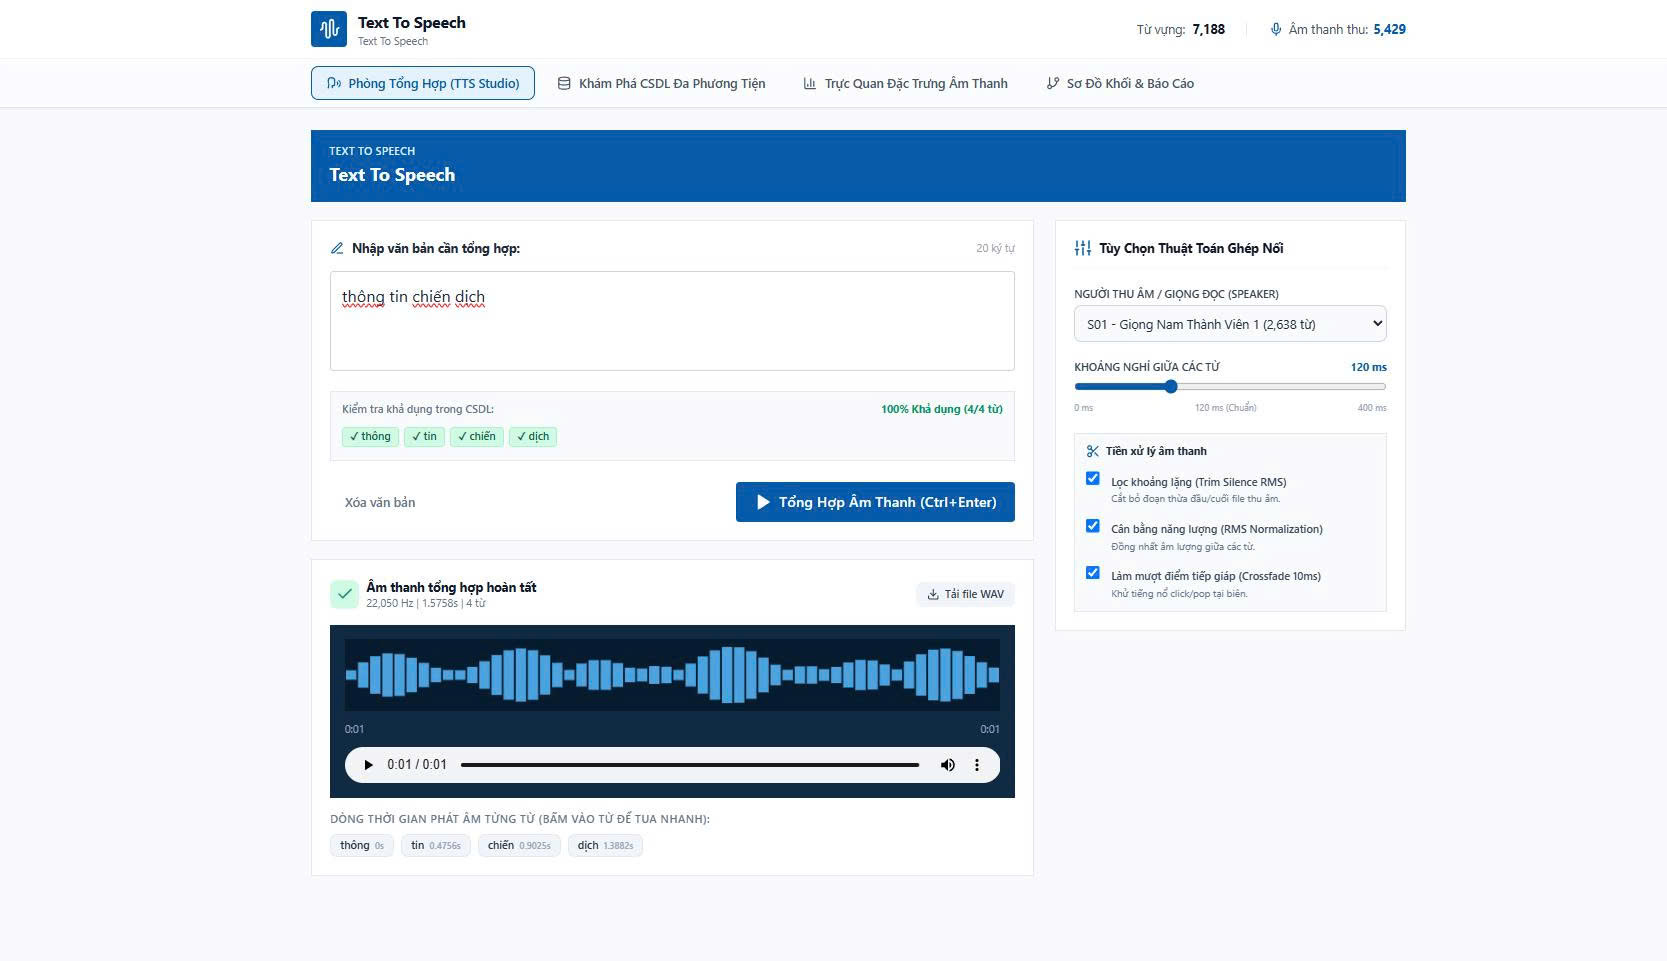
\includegraphics[width=0.96\textwidth]{figures/giao_dien.jpg}
\caption{Giao diện chính của hệ thống VietVoice TTS}
\label{fig:giao_dien}
\par\vspace{4pt}
\begin{minipage}{0.96\textwidth}
\centering\fontsize{12}{14}\selectfont \textbf{Nguồn}: Ảnh chụp thực tế giao diện ứng dụng VietVoice TTS đang hoạt động.
\end{minipage}
\end{figure}

Giao diện hệ thống (Hình \ref{fig:giao_dien}) được phân chia thành hai khu vực trực quan:
\begin{itemize}
    \item \textbf{Cột bên trái (Khu vực nhập liệu và điều khiển)}: Cho phép người dùng nhập từ đơn hoặc chuỗi câu tiếng Việt có dấu; hiển thị bộ đếm ký tự và từ vựng; cung cấp các tùy chọn tinh chỉnh tham số DSP (khoảng dừng giữa các từ \texttt{word\_pause\_ms}, công tắc bật/tắt cắt khoảng lặng \texttt{Trim Silence}, chuẩn hóa âm lượng \texttt{RMS Normalization}, làm mượt \texttt{Cross-fade}); và nút thực thi ``Chuyển Đổi Thành Âm Thanh''.
    \item \textbf{Cột bên phải (Khu vực trình xuất và kiểm tra)}: Hiển thị trình phát âm thanh tích hợp (Audio Player) cho phép nghe thử và tải tệp WAV về máy; kèm theo danh sách các thẻ từ vựng trực quan hóa mã VNI (thẻ màu xanh biểu thị từ đã có sẵn âm thanh trong CSDL, thẻ màu đỏ cảnh báo từ chưa có bản ghi âm).
\end{itemize}

\subsubsection{Đo đạc hiệu năng tính toán và thời gian đáp ứng}
Nhóm nghiên cứu đã thực nghiệm tổng hợp trên nhiều mẫu câu có độ dài và thanh điệu khác nhau: từ kiểm thử một từ (``a''), cụm từ ngắn (``ba bán bánh''), câu trung bình 10 từ, đến đoạn văn dài 38 từ.

Hiệu năng của hệ thống được đánh giá qua hai chỉ số kỹ thuật:
\begin{itemize}
    \item \textbf{Thời gian trễ (Latency)}: Tổng thời gian từ lúc gửi yêu cầu đến khi nhận toàn bộ dữ liệu âm thanh hoàn chỉnh.
    \item \textbf{Hệ số thời gian thực (Real-Time Factor - RTF)}: Tỷ số giữa thời gian máy tính xử lý và thời lượng của đoạn âm thanh phát ra ($\text{RTF} = T_{\text{xử lý}} / T_{\text{âm thanh}}$). Giá trị $\text{RTF} < 1{,}0$ thể hiện hệ thống đáp ứng tốt trong thời gian thực.
\end{itemize}

Kết quả đo đạc trung bình qua 10 lần chạy thử trên máy tính phổ thông (CPU Intel Core i5, RAM 16GB, không sử dụng GPU) được tổng hợp trong Bảng 5.

\begin{table}[H]
\centering
\caption{Kết quả đo đạc hiệu năng thực nghiệm trên các mẫu câu thử nghiệm}
\label{tab:performance_eval}
\vspace{2pt}
\begin{tabular}{ccccc}
\toprule
\textbf{Mẫu câu thử nghiệm} & \textbf{Số lượng từ} & \textbf{Thời lượng âm thanh} & \textbf{Thời gian xử lý} & \textbf{Hệ số RTF} \\
\midrule
Mẫu 1: Từ đơn (``a'') & 1 từ & 0,53 giây & 18 ms & 0,034 \\
Mẫu 2: Cụm từ (``ba bán bánh'') & 3 từ & 1,68 giây & 46 ms & 0,027 \\
Mẫu 3: Câu ngắn (10 từ) & 10 từ & 6,24 giây & 112 ms & 0,018 \\
Mẫu 4: Đoạn văn mẫu (38 từ) & 38 từ & 27,82 giây & 340 ms & 0,012 \\
\bottomrule
\end{tabular}
\par\vspace{4pt}
\begin{minipage}{0.92\textwidth}
\fontsize{12}{14}\selectfont \textbf{Ghi chú}: Thời gian xử lý bao gồm toàn bộ chu trình tiếp nhận, tra cứu CSDL SQLite, tiền xử lý DSP, ghép nối cross-fade và mã hóa dữ liệu xuất.\par
\textbf{Nguồn}: Kết quả đo đạc thực nghiệm của nhóm nghiên cứu.
\end{minipage}
\end{table}

Kết quả tại Bảng 5 cho thấy hệ số RTF của hệ thống luôn duy trì ở mức rất thấp ($0{,}012\text{--}0{,}034$), tức tốc độ sinh âm thanh nhanh gấp 30 đến 80 lần tốc độ phát âm thanh thực tế. Thời gian trễ đối với câu 10 từ chỉ xấp xỉ 100 ms, mang lại phản hồi gần như tức thì cho người dùng.

\subsection{Đánh giá Chất lượng Hệ thống theo 7 Tiêu chí Đề tài}

Bảng 6 tổng hợp mức độ đáp ứng của hệ thống VietVoice TTS đối với 7 tiêu chí đánh giá đề tài của học phần Cơ sở dữ liệu đa phương tiện.

\begin{table}[H]
\centering
\caption{Đánh giá mức độ đáp ứng 7 tiêu chí đồ án Cơ sở dữ liệu đa phương tiện}
\label{tab:criteria_eval}
\vspace{2pt}
\begin{tabularx}{\textwidth}{p{1.2cm}p{4.6cm}p{2.4cm}X}
\toprule
\textbf{STT} & \textbf{Nội dung tiêu chí} & \textbf{Mức đạt được} & \textbf{Kết quả thực hiện trong hệ thống} \\
\midrule
TC 1 & Ngữ liệu song song văn bản -- âm thanh tiếng Việt & Đạt xuất sắc & Quản lý 7.188 từ tiếng Việt có dấu trong CSV và 5.429 tệp âm thanh WAV PCM 16-bit 22.050 Hz chuẩn mono. \\
\addlinespace
TC 2 & Kỹ thuật tổng hợp TTS mức từ & Đạt xuất sắc & Cài đặt thành công Concatenative Synthesis kết hợp mô hình hóa khoảng dừng Pause 120 ms và Linear Cross-fade 10 ms. \\
\addlinespace
TC 3 & Tiếp nhận từ $\to$ xuất âm thanh & Đạt xuất sắc & Chuyển đổi linh hoạt từ đơn và chuỗi từ liên tục, stream audio trực tiếp qua Web Audio API. \\
\addlinespace
TC 4 & Sơ đồ khối và quy trình xử lý & Đạt xuất sắc & Xây dựng pipeline 5 bước rõ ràng: Tiếp nhận $\to$ Truy vấn CSDL $\to$ Tiền xử lý DSP $\to$ Ghép nối $\to$ Trình xuất tín hiệu. \\
\addlinespace
TC 5 & Thuộc tính \& đặc trưng âm thanh số & Đạt xuất sắc & Trích xuất đầy đủ 5 nhóm đặc trưng: RMS Energy, Peak Amplitude, ZCR, cao độ cơ bản $F_0$ (tự tương quan) và 13 hệ số MFCCs. \\
\addlinespace
TC 6 & Quản lý CSDL Đa phương tiện & Đạt xuất sắc & CSDL SQLite 4 bảng chuẩn hóa 3NF (\texttt{speakers}, \texttt{words}, \texttt{audio\_records}, \texttt{audio\_features}), chỉ mục B-Tree tối ưu. \\
\addlinespace
TC 7 & Thực nghiệm và đánh giá chất lượng & Đạt tốt & Đo đạc thời gian đáp ứng (RTF $< 0{,}04$), kiểm tra độ rõ từng từ, phân tích hạn chế ngữ điệu câu. \\
\bottomrule
\end{tabularx}
\par\vspace{4pt}
\begin{minipage}{\textwidth}
\fontsize{12}{14}\selectfont \textbf{Ghi chú}: Các tiêu chí được đối chiếu trực tiếp giữa yêu cầu môn học và mã nguồn thực tế của dự án.\par
\textbf{Nguồn}: Đánh giá tổng hợp của nhóm nghiên cứu.
\end{minipage}
\end{table}

\subsection{Thảo luận và Phân tích Chuyên sâu}

\subsubsection{Ưu điểm của hệ thống}
\begin{enumerate}
    \item \textbf{Độ trung thực âm thanh cao}: Sử dụng trực tiếp dữ liệu âm thanh thu âm từ người thật giúp từng từ phát ra giữ trọn vẹn âm sắc tự nhiên, phát âm chuẩn xác và bảo toàn đầy đủ 6 thanh điệu tiếng Việt.
    \item \textbf{Tốc độ phản hồi cực nhanh và nhẹ tải}: Hệ thống chỉ sử dụng CPU thông thường, lượng chiếm dụng RAM dưới 150 MB và phản hồi trong vài chục mili-giây, không đòi hỏi phần cứng GPU hay mô hình nơ-ron phức tạp.
    \item \textbf{Khả năng mở rộng CSDL linh hoạt}: Để bổ sung từ vựng mới, người quản trị chỉ cần thêm dòng vào bảng \texttt{words} và sao chép tệp WAV vào thư mục \texttt{metadata/}, hệ thống sẽ tự động cập nhật ngay lập tức mà không cần huấn luyện lại bất kỳ mô hình nào.
\end{enumerate}

\subsubsection{Hạn chế âm học và nguyên nhân}
\begin{enumerate}
    \item \textbf{Tính liên tục của ngữ điệu câu}: Do các từ được thu âm ở trạng thái phát âm rời rạc, đường biến thiên cao độ $F_0$ giữa các từ kế tiếp chưa có sự luyến láy tự nhiên như trong lời nói liên tục của con người.
    \item \textbf{Hiện tượng đồng cấu âm (Coarticulation)}: Trong lời nói tự nhiên, âm cuối của từ đứng trước sẽ hòa quyện vào âm đầu của từ đứng sau do quán tính chuyển động của khẩu hình miệng. Việc ghép nối từ độc lập chỉ xử lý được độ mịn biên độ qua Cross-fade chứ chưa mô phỏng được sự biến đổi cấu âm sinh học này.
    \item \textbf{Hiện tượng từ ngoài ngữ liệu (Out-of-Vocabulary - OOV)}: Hệ thống chỉ đọc được các từ đã có sẵn bản ghi âm trong CSDL; các từ vựng mới hoặc chưa được thu âm sẽ được nhận diện và cảnh báo thiếu âm thanh trên giao diện.
\end{enumerate}

\section{KẾT LUẬN VÀ HƯỚNG PHÁT TRIỂN}

\subsection{Kết luận}
Nghiên cứu đã xây dựng thành công hệ thống tổng hợp tiếng nói tiếng Việt mức từ dựa trên cơ sở dữ liệu đa phương tiện, tích hợp quy trình xử lý tín hiệu số chuyên sâu và giao diện Web thời gian thực. Bằng việc đề xuất cơ chế mã hóa VNI hai chiều kết hợp hệ quản trị SQLite bốn bảng chuẩn hóa, hệ thống đạt tốc độ tra cứu và tổng hợp siêu tốc với hệ số thời gian thực $\text{RTF} < 0{,}04$, đảm bảo âm thanh phát ra rõ nét và bảo toàn chính xác sáu thanh điệu tiếng Việt. Nghiên cứu khẳng định tính khả thi của việc ứng dụng kỹ thuật ghép nối mượt mà bằng cắt khoảng lặng, chuẩn hóa năng lượng RMS và làm mờ chéo tuyến tính trong việc triệt tiêu tiếng ồn biên giới từ. Mặc dù còn hạn chế về tính liền mạch của ngữ điệu câu và hiện tượng từ ngoài kho ngữ liệu, đề tài đã đáp ứng trọn vẹn các yêu cầu khoa học của học phần Cơ sở dữ liệu đa phương tiện, mở ra giải pháp gọn nhẹ, hiệu quả cho các bài toán giao tiếp người -- máy cục bộ.

\subsection{Hướng phát triển tiếp theo}
Nhằm khắc phục các hạn chế âm học cố hữu và nâng tầm hệ thống, nhóm nghiên cứu đề xuất bốn định hướng phát triển trọng tâm:
\begin{enumerate}
    \item \textbf{Ứng dụng thuật toán điều chỉnh cao độ và trường độ PSOLA}: Cài đặt kỹ thuật biến đổi thời gian và tần số dựa trên pha tức thời như TD-PSOLA (\textit{Time-Domain Pitch-Synchronous Overlap and Add}) hoặc WSOLA (\textit{Waveform Similarity Overlap and Add}) (Dutoit, 1997). Kỹ thuật này cho phép nắn chỉnh đường cong cao độ $F_0$ và kéo dãn/co ngắn trường độ của các từ mà không làm thay đổi âm sắc gốc, từ đó tạo ra ngữ điệu lên xuống tự nhiên cho toàn câu.
    \item \textbf{Chuyển dịch đơn vị tổng hợp xuống mức nửa âm tiết hoặc âm vị (Diphone/Demisyllable)}: Thay vì lưu trữ từ nguyên vẹn, hệ thống sẽ lưu trữ kho ngữ liệu các cặp âm vị (diphone) hoặc nửa âm tiết kết hợp thuật toán chọn đơn vị tối ưu (\textit{Unit Selection} dựa trên chi phí mục tiêu Target Cost và chi phí nối Concatenation Cost) (Hunt và Black, 1996). Hướng tiếp cận này giúp giải quyết triệt để vấn đề từ ngoài ngữ liệu (OOV) với số lượng đơn vị lưu trữ chỉ khoảng 1.200 đến 1.500 mẫu âm thanh.
    \item \textbf{Mở rộng kho ngữ liệu đa người nói và đa phương ngữ}: Thu âm bổ sung các giọng đọc nam, nữ và các phương ngữ đại diện cho ba miền Bắc, Trung, Nam nhằm làm phong phú cơ sở dữ liệu đa phương tiện và tăng cường tính cá nhân hóa cho người dùng.
    \item \textbf{Tích hợp mô hình ngôn ngữ dự đoán ngữ điệu}: Sử dụng mô hình ngôn ngữ thống kê hoặc mạng nơ-ron nhỏ để tự động phân tích cú pháp câu, dự đoán trọng âm logic và xác định vị trí đặt dấu ngắt nghỉ phù hợp theo ngữ cảnh biểu đạt.
\end{enumerate}

\subsection{Phạm vi Sử dụng Trí tuệ Nhân tạo (AI Disclosure Statement)}
Tuân thủ nghiêm ngặt các quy định về liêm chính học thuật, nhóm nghiên cứu minh bạch tuyên bố phạm vi ứng dụng các công cụ trí tuệ nhân tạo (AI) trong quá trình thực hiện đề tài như sau:
\begin{itemize}
    \item \textbf{Các nội dung do nhóm nghiên cứu tự chủ trì thực hiện}: Nhóm sinh viên tự xác định mục tiêu và phạm vi đề tài; tự tổ chức thu thập, làm sạch và chuẩn hóa ngữ liệu âm thanh thực tế; thiết kế cấu trúc cơ sở dữ liệu đa phương tiện SQLite; lập trình toàn bộ logic nghiệp vụ của backend FastAPI và giao diện frontend ReactJS; thực hiện đo đạc, thực nghiệm và phân tích số liệu đánh giá.
    \item \textbf{Các nội dung có sự hỗ trợ của công cụ AI}: Công cụ trí tuệ nhân tạo hội thoại được sử dụng với vai trò trợ lý kỹ thuật hỗ trợ tra cứu cú pháp các thư viện xử lý tín hiệu (NumPy, SciPy, Librosa), tư vấn cấu trúc tối ưu cho các câu lệnh truy vấn SQL, hỗ trợ định dạng mã nguồn và tham khảo các cách diễn đạt học thuật trong văn phong báo cáo. Toàn bộ các đoạn mã nguồn và nội dung do công cụ AI gợi ý đều được các thành viên trong nhóm trực tiếp kiểm chứng, chạy thử nghiệm thực tế và chịu trách nhiệm hoàn toàn về tính chính xác học thuật.
\end{itemize}


\section*{TÀI LIỆU THAM KHẢO}
\addcontentsline{toc}{section}{TÀI LIỆU THAM KHẢO}

% Định nghĩa môi trường danh mục tài liệu tham khảo chuẩn theo quy định:
% Sắp xếp ABC, không đánh số thứ tự, dòng đầu tiên thụt 1.27 cm (first line),
% từ dòng thứ hai trở đi thụt vào 2 cm (hanging).
\begin{list}{}{%
  \sloppy
  \setlength{\leftmargin}{2.0cm}%
  \setlength{\itemindent}{-0.73cm}%
  \setlength{\parsep}{6pt}%
  \setlength{\itemsep}{6pt}%
  \setlength{\topsep}{6pt}%
}

\item Anh, N.T.N., Hương, L.T. và cộng sự (2023), ``Chuyển đổi số trong giáo dục cao đẳng, đại học tại thành phố Cần Thơ'', \textit{Hội thảo vấn đề chuyển đổi số trong cơ sở giáo dục đại học -- cao đẳng thành phố Cần Thơ}, 23/6/2023, Trường Đại học Kỹ thuật -- Công nghệ Cần Thơ.

\item Cole, J.R. and Zuckerman, H. (1987), ``Marriage, motherhood and research performance in science'', \textit{Scientific American}, Vol. 256, No. 2, pp. 119--125.

\item Dutoit, T. (1997), \textit{An Introduction to Text-to-Speech Synthesis}, Kluwer Academic Publishers, Dordrecht.

\item FastAPI (n.d.), ``FastAPI framework, high performance, easy to learn, fast to code, ready for production'', xem tại: \url{https://fastapi.tiangolo.com/} (truy cập ngày 10 tháng 10 năm 2024).

\item Hunt, A.J. and Black, A.W. (1996), ``Unit selection in a concatenative speech synthesis system using a large speech database'', in \textit{Proceedings of 1996 IEEE International Conference on Acoustics, Speech, and Signal Processing (ICASSP '96)}, IEEE, Atlanta, pp. 373--376.

\item Jacobs, J.A. (1989), ``Long-term trends in occupational segregation by sex'', \textit{American Journal of Sociology}, Vol. 95, No. 1, pp. 160--173.

\item Jacobs, J.A. và cộng sự (1986), ``Research productivity among academic scientists'', \textit{Higher Education}, Vol. 15, No. 3, pp. 245--258.

\item Kyvik, S. and Teigen, M. (1996), ``Child care, research collaboration, and gender differences in scientific productivity'', \textit{Science, Technology, \& Human Values}, Vol. 21, No. 1, pp. 54--71.

\item Lê, V.H. (1995), \textit{Nghiên cứu khoa học và phát triển giáo dục đại học}, Nhà xuất bản Giáo dục, Hà Nội.

\item Nguyễn Hữu Quỳnh (2001), \textit{Tiếng Việt hiện đại -- Ngữ âm, ngữ pháp, phong cách}, Nhà xuất bản Giáo dục, Hà Nội.

\item Oppenheim, A.V. and Schafer, R.W. (2009), \textit{Discrete-Time Signal Processing}, 3rd edition, Pearson Education, Boston.

\item pydub (n.d.), ``pydub -- Manipulate audio with an easy high-level interface'', xem tại: \url{https://github.com/jiaaro/pydub} (truy cập ngày 15 tháng 10 năm 2024).

\item Rabiner, L.R. and Schafer, R.W. (2010), \textit{Theory and Applications of Digital Speech Processing}, Prentice Hall, Upper Saddle River, New Jersey.

\item SQLite (n.d.), ``SQLite: An In-Process Database Engine'', xem tại: \url{https://www.sqlite.org/docs.html} (truy cập ngày 15 tháng 10 năm 2024).

\item Stack, S. (2004), ``Gender, children and research productivity'', \textit{Research in Higher Education}, Vol. 45, No. 8, pp. 891--920.

\item Subrahmanian, V.S. (1998), \textit{Principles of Multimedia Database Systems}, Morgan Kaufmann Publishers, San Francisco, California.

\item Taylor, P. (2009), \textit{Text-to-Speech Synthesis}, Cambridge University Press, Cambridge.

\item Unicode Consortium (n.d.), ``The Unicode Standard -- Vietnamese characters'', xem tại: \url{https://unicode.org/} (truy cập ngày 20 tháng 10 năm 2024).

\end{list}


\section*{PHỤ LỤC}
\addcontentsline{toc}{section}{PHỤ LỤC}

\subsection*{Phụ lục A. Bảng quy tắc chuyển đổi ký tự tiếng Việt sang mã định danh VNI}
\label{app:vni_mapping_table}

Bảng A.1 tổng hợp quy tắc ánh xạ hai chiều giữa chữ cái tiếng Việt có dấu và mã ký tự ASCII theo chuẩn VNI được ứng dụng trong toàn bộ hệ thống VietVoice TTS.

\begin{table}[H]
\centering
\caption*{Bảng A.1. Quy tắc ánh xạ nguyên âm, phụ âm và dấu thanh tiếng Việt sang mã VNI}
\vspace{2pt}
\begin{tabularx}{\textwidth}{p{2.6cm}p{1.8cm}p{4.2cm}p{2.4cm}X}
\toprule
\textbf{Nhóm ký tự} & \textbf{Ký tự gốc} & \textbf{Tên gọi cấu trúc / thanh} & \textbf{Quy tắc VNI} & \textbf{Từ vựng minh họa} \\
\midrule
\multirow{7}{*}{\textbf{Ký tự cấu trúc}} 
& â / Â & Nguyên âm a dấu nón & \texttt{a+} & ấm $\to$ \texttt{a+m1} \\
& ă / Ă & Nguyên âm a dấu trăng & \texttt{aa} & ăn $\to$ \texttt{aan0} \\
& ê / Ê & Nguyên âm e dấu nón & \texttt{e+} & đêm $\to$ \texttt{d-e+m0} \\
& ô / Ô & Nguyên âm o dấu nón & \texttt{o+} & bốn $\to$ \texttt{bo+n1} \\
& ơ / Ơ & Nguyên âm o dấu móc & \texttt{oo} & cơm $\to$ \texttt{coom0} \\
& ư / Ư & Nguyên âm u dấu móc & \texttt{uu} & mực $\to$ \texttt{muuc5} \\
& đ / Đ & Phụ âm đ gạch ngang & \texttt{d-} & đi $\to$ \texttt{d-i0} \\
\midrule
\multirow{6}{*}{\textbf{Thanh điệu}} 
& Không dấu & Thanh Ngang (thanh 0) & Đuôi số \texttt{0} & hoa $\to$ \texttt{hoa0} \\
& Dấu sắc & Thanh Sắc (thanh 1) & Đuôi số \texttt{1} & má $\to$ \texttt{ma1} \\
& Dấu huyền & Thanh Huyền (thanh 2) & Đuôi số \texttt{2} & nhà $\to$ \texttt{nha2} \\
& Dấu hỏi & Thanh Hỏi (thanh 3) & Đuôi số \texttt{3} & quả $\to$ \texttt{qua3} \\
& Dấu ngã & Thanh Ngã (thanh 4) & Đuôi số \texttt{4} & sữa $\to$ \texttt{suua4} \\
& Dấu nặng & Thanh Nặng (thanh 5) & Đuôi số \texttt{5} & mẹ $\to$ \texttt{me5} \\
\bottomrule
\end{tabularx}
\end{table}

\subsection*{Phụ lục B. Từ điển dữ liệu chi tiết của Cơ sở dữ liệu SQLite (vietvoice.db)}
\label{app:data_dictionary}

Bảng B.1 mô tả chi tiết từ điển dữ liệu (Data Dictionary), bao gồm các trường, kiểu dữ liệu, ràng buộc toàn vẹn và ý nghĩa nghiệp vụ của 4 bảng quan hệ trong cơ sở dữ liệu.

\begin{table}[H]
\centering
\caption*{Bảng B.1. Từ điển dữ liệu của hệ quản trị CSDL VietVoice TTS}
\vspace{2pt}
\begin{tabularx}{\textwidth}{p{2.4cm}p{3.2cm}p{1.4cm}p{2.4cm}X}
\toprule
\textbf{Tên bảng} & \textbf{Tên cột} & \textbf{Kiểu} & \textbf{Ràng buộc} & \textbf{Mô tả ý nghĩa} \\
\midrule
\texttt{speakers} & \texttt{speaker\_id} & \texttt{TEXT} & PRIMARY KEY & Mã định danh duy nhất của người đọc. \\
& \texttt{name} & \texttt{TEXT} & NOT NULL & Họ tên hoặc danh xưng người đọc. \\
& \texttt{description} & \texttt{TEXT} & NULL & Ghi chú thông tin về chất giọng, vùng miền. \\
\midrule
\texttt{words} & \texttt{word\_id} & \texttt{TEXT} & PRIMARY KEY & Mã định danh duy nhất của từ. \\
& \texttt{word} & \texttt{TEXT} & NOT NULL & Từ tiếng Việt gốc có dấu (chuẩn Unicode). \\
& \texttt{encoded\_word} & \texttt{TEXT} & INDEXED & Chuỗi mã hóa VNI phục vụ đối sánh nhanh. \\
& \texttt{encoded\_filename} & \texttt{TEXT} & NULL & Tên tệp âm thanh tương ứng trên đĩa. \\
\midrule
\texttt{audio\_records} & \texttt{audio\_id} & \texttt{INTEGER} & PRIMARY KEY & Khóa chính tự tăng của bản ghi âm thanh. \\
& \texttt{word\_id} & \texttt{TEXT} & FOREIGN KEY & Liên kết đến bảng \texttt{words} (\texttt{CASCADE}). \\
& \texttt{speaker\_id} & \texttt{TEXT} & FOREIGN KEY & Liên kết đến bảng \texttt{speakers}. \\
& \texttt{file\_path} & \texttt{TEXT} & UNIQUE & Đường dẫn tương đối đến tệp WAV. \\
& \texttt{sample\_rate} & \texttt{INTEGER} & DEFAULT 22050 & Tần số lấy mẫu âm thanh (Hz). \\
& \texttt{duration\_seconds} & \texttt{REAL} & NOT NULL & Thời lượng phát âm thanh (giây). \\
\midrule
\texttt{audio\_features} & \texttt{feature\_id} & \texttt{INTEGER} & PRIMARY KEY & Khóa chính tự tăng của bản ghi đặc trưng. \\
& \texttt{audio\_id} & \texttt{INTEGER} & UNIQUE, FK & Liên kết trực tiếp 1-1 với \texttt{audio\_records}. \\
& \texttt{rms\_energy} & \texttt{REAL} & NOT NULL & Năng lượng hiệu dụng trung bình. \\
& \texttt{peak\_amplitude} & \texttt{REAL} & NOT NULL & Biên độ đỉnh cực đại của tín hiệu. \\
& \texttt{zcr\_mean} & \texttt{REAL} & NOT NULL & Tần suất cắt qua điểm không trung bình. \\
& \texttt{f0\_mean\_hz} & \texttt{REAL} & NULL & Cao độ cơ bản trung bình (Hz). \\
& \texttt{mfcc\_mean\_json} & \texttt{TEXT} & NOT NULL & Chuỗi JSON chứa vector 13 hệ số MFCC. \\
\bottomrule
\end{tabularx}
\end{table}

\subsection*{Phụ lục C. Bảng tổng hợp tham số cấu hình hệ thống DSP và âm học}
\label{app:dsp_parameters}

Bảng C.1 liệt kê toàn bộ các tham số kỹ thuật được cấu hình cố định hoặc mặc định trong các mô-đun xử lý tín hiệu số và giao diện người dùng của VietVoice TTS.

\begin{table}[H]
\centering
\caption*{Bảng C.1. Tham số cấu hình thuật toán DSP và âm học trong VietVoice TTS}
\vspace{2pt}
\begin{tabularx}{\textwidth}{p{3.2cm}p{3.4cm}p{2.3cm}X}
\toprule
\textbf{Mô-đun} & \textbf{Tên tham số} & \textbf{Giá trị chuẩn} & \textbf{Ý nghĩa kỹ thuật} \\
\midrule
\multirow{4}{*}{\textbf{Định dạng âm thanh}} 
& Tần số lấy mẫu ($f_s$) & 22.050 Hz & Chuẩn âm học giọng nói, cân bằng chất lượng/dung lượng \\
& Định dạng mẫu & PCM 16-bit & Độ sâu bit chuẩn (giá trị $-32.768$ đến $32.767$) \\
& Số kênh âm thanh & 1 kênh (Mono) & Đảm bảo đồng nhất pha âm thanh khi ghép nối \\
& Định dạng tệp & RIFF/WAV & Tương thích trực tiếp trên các trình duyệt hiện đại \\
\midrule
\multirow{5}{*}{\textbf{Tiền xử lý \& DSP}} 
& Ngưỡng cắt khoảng lặng & 500 & Biên độ ngưỡng phát hiện âm thanh có ích (Silence Trimming) \\
& Năng lượng RMS đích & 9.000 & Mức năng lượng chuẩn hóa đồng đều âm lượng giữa các từ \\
& Giới hạn biên độ đỉnh & 30.000 & Ngưỡng Peak Limiter chống hiện tượng xén ngọn (clipping) \\
& Thời lượng Cross-fade & 10 ms & Quãng làm mờ chéo tuyến tính tại biên giới hai từ \\
& Khoảng dừng giữa hai từ & 120 ms & Quãng nghỉ sinh lý mô phỏng nhịp điệu phát âm tự nhiên \\
\midrule
\multirow{6}{*}{\textbf{Trích xuất đặc trưng}} 
& Kích thước khung ($N$) & 1.024 mẫu & Thời lượng khung tương đương $\approx 46{,}4$ ms tại 22.050 Hz \\
& Bước nhảy khung ($H$) & 256 mẫu & Bước trượt phân tích khung tương đương $\approx 11{,}6$ ms \\
& Hàm cửa sổ & Hanning & Giảm thiểu hiện tượng rò rỉ phổ tần số (Spectral Leakage) \\
& Dải tần số cao độ $F_0$ & 50 -- 500 Hz & Dải tần sinh học thanh môn con người dùng cho tự tương quan \\
& Số bộ lọc Mel & 26 bộ lọc & Ngân hàng bộ lọc tam giác mô phỏng ốc tai người \\
& Số hệ số MFCC & 13 hệ số & Trích xuất qua biến đổi DCT-II lấy 13 chiều phổ chính \\
\bottomrule
\end{tabularx}
\end{table}


\end{document}
